\documentclass{VUMIFPSkursinis}
\usepackage{algorithmicx}
\usepackage{algorithm}
\usepackage{algpseudocode}
\usepackage{amsfonts}
\usepackage{amsmath}
\usepackage{bm}
\usepackage{caption}
\usepackage{color}
\usepackage{float}
\usepackage{graphicx}
\usepackage{listings}
\usepackage{subfig}
\usepackage{wrapfig}

% Titulinio aprašas
\university{Vilniaus universitetas}
\faculty{Matematikos ir informatikos fakultetas}
\department{Matematinės informatikos katedra}
\papertype{Tiriamojo seminaro darbas}
\title{Nesudėtingų robotų konstravimas ir programavimas}
\status{3 kurso  studentai}
\author{Anastasija Kiseliova}
\secondauthor{Karolis Šimaitis} 
\supervisor{lekt. Irus Grinis}
\date{Vilnius – \the\year}

\bibliography{bibliografija}

\begin{document}
\maketitle
\tableofcontents

\sectionnonum{Įvadas}
Žmonės visais laikais siekė peržengti savo fizinių galimybių ribas. Puikus to pavyzdys - legenda apie Ikarą bei Dedalą. Galbūt anuomet tokia idėja ir skambėjo kaip fikcija, tačiau šiais laikais esame pasiekę daugiau, nei bet kada anksčiau. Robotika - mokslas, apjungiantis savyje mechanikos inžineriją, elektros inžineriją, kompiuterių mokslą bei daug kitų disciplinų, leidžia kurti tai, apie ką mūsų protėviai galėjo tik pasvajoti. Tai, kas leidžia pasiekti padanges.\par
Ornitopteris - (ornito- + gr. pteron - sparnas) - aparatas, kuris skraidymui pasitelkia plasnojančius sparnus. Šio tipo prietaiso dizainų yra įvairių. Geriausiai žinomas, tikriausiai, yra Leonardo Da Vinčio paliktas modelis. Jo mašina turėjo būti sukurta skraidyti žmogui, ir, nors tokių įtaisų šiais laikais taip pat esama, pristatysime daug mažesnio dydžio analogą. MAV (Micro Aerial Vehicles) tyrinėjimas yra pakankamai nauja sritis. Elektronikos komponenčių, pavyzdžiui, elektrinių motorų mažėjimas ir mikroelektronikos tobulėjimas lėmė per paskutinius keis metus išaugusį susidomėjimą ja. Dabar kiekvienas gali namie gana pigiai pasidaryti miniatiūrinį lėktuvą ar sraigtasparnį. Kam? Nedideli ornitopteriai gali būti panaudojami patalpų viduje, pavyzdžiui, daiktų paieškai, arba saugumui užtikrinti. Išorėje jie panaudojami ornitologų. Kadangi savo išvaizda ir dydžiu primena paukščius, įsilieję į pulką ornitopteriai geba stebėti jų elgesį, migraciją. Pagrindinė šių robotų savybė ir yra aplinkos stebėjimas iš paukščio skrydžio. Ornitopteriai taip pat kuriami siekiant ištirti plasnojančių sparnų aerodinamiką. \par
Taigi, tiriamojo seminaro darbo tikslas - susipažinti su robotų konstravimu bei programavimu; pagaminti roboto - ornitopterio, prototipą. 

\section{Aerodinamika}
Kaip ornitopteris sukuria keliamąją ir varomąsias jėgas, nors jis plasnoja į abi puses? Šį klausimą aprašo ir bando pateikti atsakymą Horst Räbiger savo knygoje, kuria dalinai remsimės savo ornitopteriui tobulinti. Knygoje pateiktos išvados remiasi įvairiais žinomais tyrimais. Be plasnojimo aerodinamikos, taip pat turime įvertinti ir plasnojančio sparno dinamiką.

\subsection{Ornitopterio plasnojimo dinamikos schema}
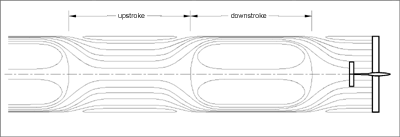
\includegraphics{img/vortex}\\

\subsection{Sparnų aerodinamikos skaičiavimai}
Visų pirma, sparnas yra menamai padalinamas į labai siauras juosteles. Tada kiekvienai iš šių juostelių apskaičiuojamas aerodinaminės jegos pastoviomis oro tekmės sąlygomis. Jų suma yra viso sparno pločio integralas.
Šitaip gauname kilimo ir varomąsias jėgas plasnojančiam sparnui kuriuo nors fiksuotu laiko momentu plasnojimo cikle.
Šis procesas yra kartojamas lygiais laiko tarpais sparnų mosavimo judesiui, todėl tokie dalykai kaip cirkuliacijos pokyčiai ir ateinančio oro srauto pokyčiai tampa pagrindo dalimi. Tuo pat metu yra laikoma, kad oro tekmė skaičiavimų metu nesikeičia .
Viso mosto jėgą galime gauti integruodami jėgos progresiją laiko atžvilgiu. Todėl plasnojimas žemyn ir plasnojimas aukštyn apskaičiuojami atskirai ir tai sudaro viso plasnojimo ciklo sukuriamą jėga.

\subsection{Teoriniai ornitopterio aerodinaminiai duomenys}
Aerodinamikos duomenys gauti naudojantis ornitopterių aerodinamikai apskaičiuoti skirtu įrankiu Orni1\\
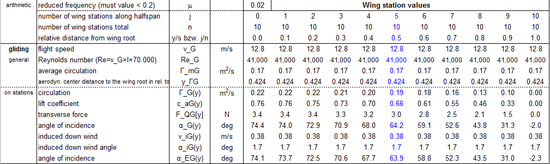
\includegraphics[scale=0.9]{img/gliding}\\
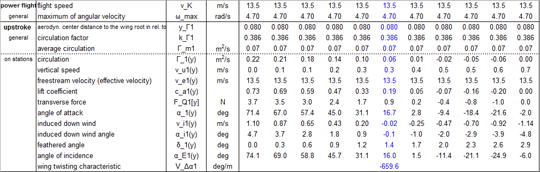
\includegraphics[scale=0.9]{img/upstroke}\\
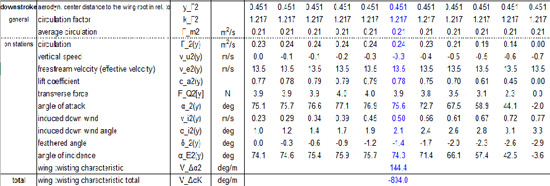
\includegraphics[scale=0.9]{img/downstroke}\\
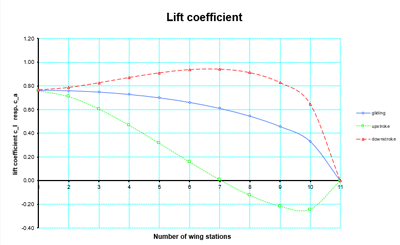
\includegraphics[scale=0.9]{img/liftforce}\\
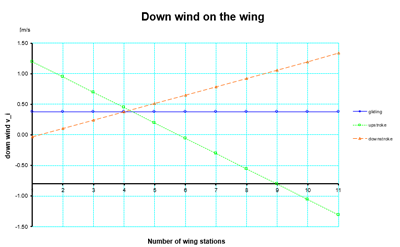
\includegraphics[scale=0.9]{img/downwind}\\
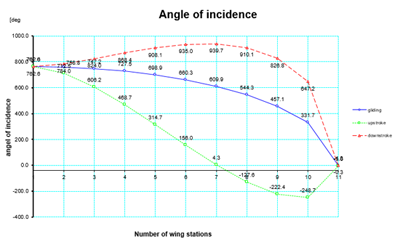
\includegraphics[scale=0.9]{img/angle}\\

\section{Ornitopterio grandinės schema}
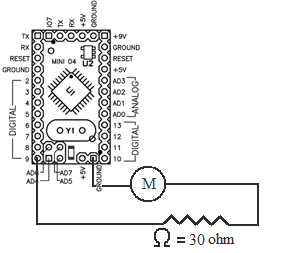
\includegraphics[scale=0.9]{img/scheme}\\

\section{Dar šiek tiek teorijos}
\subsection{Darbas su Bandomąja lenta}
Testuojant grandinę ir į ją ieinančius elementus, labai praverčia bandomoji lenta: prietaisas, leidžiantis sujungti komponentes į grandinę be papildomo litavimo. Breadbord'as yra stačiakampė plastikinė plokštė, kurioje lygiais intervalais išsidėsčiusios skylutės. Šią plokšę dažnai skiria trys grioveliai: du viršuje ir apačioje, ir vienas per vidurį. Išorinės eilės jungiasi viena su kita horizontaliai. Viena eilutė skirta teigiamai, kita neigiamai išeičiai/įeičiai. Per vidurį esančios eilės skylučiu yra skirtos komponentėms jungti. Visos skylutės, esančios viename stulpelyje, yra sujungtos. Per vidurį einantis griovelis atskiria šias dvi eiles skylučių. Naudodami bandomąją lentą galime labai paprastai viską sujungti tiek nuosekliai, tiek lygiagrečiai.\\

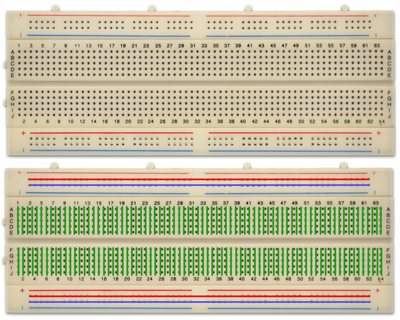
\includegraphics{img/breadboard}\\
Elementų sujungimą tarpusavy palengvina laidai su antgaliais, vadinamais „jump'eriais“. Jie būna trijų jungimo tipų: vyras/vyras, vyras/moteris, moteris/moteris. Antgalis-vyras turi metalini strypelį, kuris įkišamas į bandomosios lentos skylutes arba antgalius-moteris. Antgalis-moteris yra naudojamas kaip ir jungtis ant bandomosios lentos. Su šiuo antgaliu galime prijungti kitas elektronines detales tiesiogiai.\\
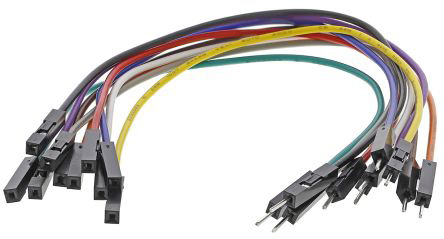
\includegraphics[scale=3]{img/jumperwire}\\

\subsection{Komponenčių fizinių duomenų matavimas naudojantis multimetru}
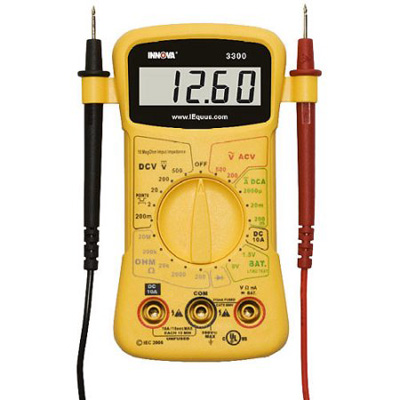
\includegraphics{img/multimeter}\\
Multimetras - įrankis, skirtas įvairiems dydžiams matuoti. Elektronikoje naudojamas multimetras dažniausiai turi šiuos matavimo rėžimus: Amperų matavimas, Voltų matavimas, Omų (varžos) matavimas ir grandinės uždarumo matavimas. Šiuolaikiniai multimetrai turi ir kitokių matavimo rėžimų, tačiau pagrindiniai išlieka paminėtieji. Matavimai atliekami taip: pirma, nustatoma multimetro padėtis į vieną iš rėžimų. Kiekvienas rėžimas skirstomas į reikšmes, iki kurių multimetras gali matuoti. Jeigu norimo matuoti dydžio reikšmė visiškai nežinoma, pradedama nuo didžiausios reikšmės ir mažinama tol, kol skaičiai priartėja prie vienos iš reikšmių arčiausiai. Antra, matavimo laidai yra pridedami prie testuojamo prietaiso/komponento galų taip, kad susidarytu grandinė. Trečia, priklausomai nuo testavimo rėžimo, galimai reikia prijungti viską prie elektros šaltinio. Jeigu multimetro ekrane rodomas klaidos pranešimas arba "1    " (skirtingi gamintojai skirtingai žymi), reiškia, kad matuojama reikšmė yra didesnė, negu pasirinkta reikšme ant multimetro. Jeigu reikšmė - nulis arba labai maža, grįžtame į pirmą žingsnį ir sumažime rėžimo reikšmę. Taip darome tol, kol pasiekiame mažiausią reikšmę, arba kai pirmą kartą pasiekiame klaidą. Pirmuoju atvėju tiksliau pamatuoti su šiuo multimetru neišeis, o kitu atvėju grįžtame į aukštesnį multimetro matavimo rėžimo tikslumą ir pamatuojame reikšmę. Tada mes esame užtikrinti, kad multimetras rodys tiksliausius rodmenis. Grandinės uždarumo rėžimas nereikalauja elektros šaltinio. Šio rėžimo metu yra siunčiama srovė iš multimetro ir laukiama jos grįžtant atgal į multimetrą. Jeigu srovė grįžta, multimetras skleidžia cypimo garsą, o jeigu ne, tai jokio garso nėra. Šio rėžimo pagalba taip pat galime nustatyti komponentų ypatingas savybes (pvz.: ar tranzistorius yra PNP, ar NPN tipo). Šių savybių nustatymo metu garsas nėra skleidžiamas, ir rodomi skaičiai ekrane. Šių skaičių reikšmė kiekvienam elementui yra skirtinga.

\section{Naudotos detalės}
Roboto karkasui panaudota detalė iš  „Nine Eagles“ motoro rinkinio sudaro pagrindinę ašį. Kitos karkaso detalės daugiausia pasirinktos tik dėl nedideli svorio tam, kad ornitopterio sparnai nebūtų per daug apkrauti (šiaudeliai, pagaliukai). Taip pat, užtikrinti saugumui, naudojamas 30Ω rezistorius. Pilnas ornitopterio ilgis - 14cm, plotis su sparnais - 29cm. 
Roboto valdymui naudojamas Arduino mikrokontroleris.

\subsection{Mikrokontroleris}
Arduino Pro Mini yra „ATmega328“ (vieno lusto mikrokontroleris) besinaudojanti mikrokontrolerio plokštė. Ji turi 14 skaitmeninių įvesties / išvesties kaiščių (iš kurių 6 gali būti naudojami kaip PWM išėjimai), 6 analoginius įėjimus, joje įrengtą rezonatorių, perkrovimo mygtuką ir angas tvirtinimui prie kaiščių. Šeši kaiščiai gali būti prijungiami prie FTDI kabelio arba USB adapterio teikti maitinimą plokštei.\cite{ArduinoDok}

\subsection{Motoras}
„Nine Eagles“ 10g sveriantis mini motoras, priimantis 3,7V ir 110mAh. „Nine Eagles“ specializuojasi dronų kūrime ir gamina itin lengvus ir sąlyginai galingus motorus.

\section{Programos kodas}

Programavimo dalis prototipe įgyvendinama minimaliai. Norint kontroliuoti motoro galią bei greitį, reikėtų prie bendros schemos pridėti tokias komponentes, kaip potenciometras. Žinoma, pilname ornitopterio modelyje turėtų būti pasiekiama absoliuti kontrolė, tai yra, skrydžio režimai įgyvendinami ne keičiant laiką tarp impulsų.\\

void loop() {\\
	
	ascend(3000);\\
	floating(1000);\\
	glide(500);\\
	descend(1500);\\
}\\

void ascend(int time){\\
	digitalWrite(motorPin, HIGH);\\
	delay(time);\\
}\\

void floating(int time){\\
	for(int i = 0; i< 100; i++){\\
		digitalWrite(motorPin, HIGH);\\
		delay(time*0.9/100);\\
		digitalWrite(motorPin, LOW);\\
		delay(time/1000);\\
	}\\
}

void glide(int time){\\
	delay(time);\\
	//Make wings parallel with the ground\\
	//Motor is completely off\\
}\\

void descend(int time){\\
	for(int i = 0; i< 100; i++){\\
		digitalWrite(motorPin, HIGH);\\
		delay(time*0.7/100);\\
		digitalWrite(motorPin, LOW);\\
		delay(time*0.3/100);\\
	}
}
\sectionnonum{Rezultatai ir išvados}
Atliekant darbą, sunkiausia dalis buvo optimaliai pasirinkti detales kuriant kūno mechaninį judėjimą. Kadangi ornitopterių konstravimas nėra plačiai paplitęs, parduotuvėje jau pagamintos dalys nėra parduodamos. Teko pasitelkti vaizduotę. \par
Prototipas buvo sukurtas po daugelio bandymų. Dizainas, prie kurio buvo pasilikta, yra optimalus turimoms priemonėms. Tęsiant projektą, reikėtų naudoti galingesnį motorą, tvirtesnį karkasą bei sparnus, prijungti uodegą skridimo krypties reguliavimui, atitinkamai pakeisti kodą.

\begin{figure}[H]
    \centering
    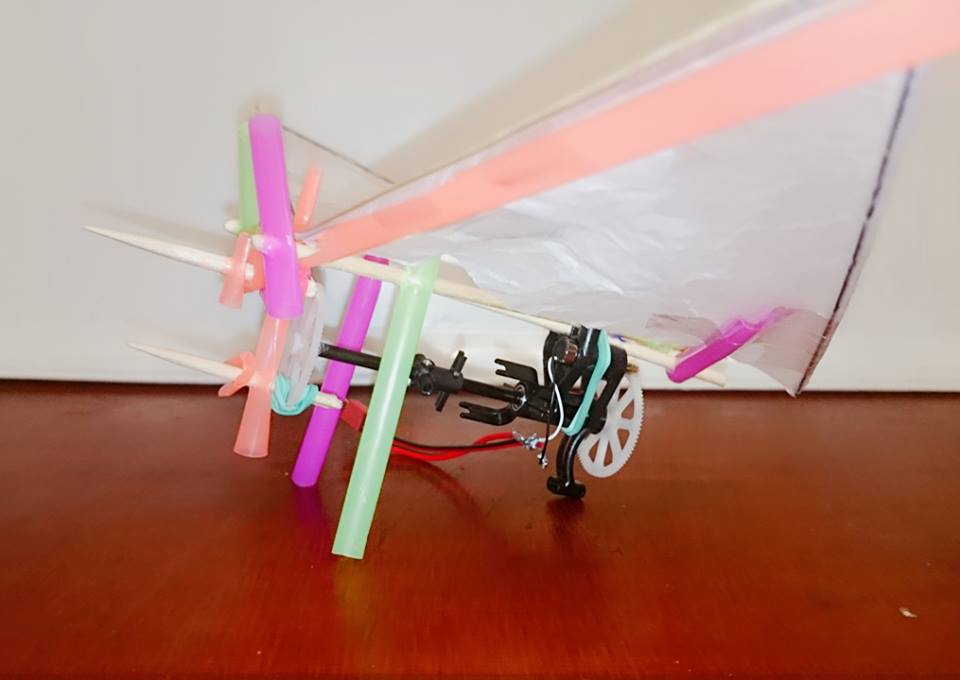
\includegraphics[scale=0.5]{img/orni}
    \caption{Prototipas}
    \label{img:mlp}
\end{figure}

https://www.youtube.com/watch?v=qNnkbspvHCc

\begin{thebibliography}{9}
	\bibitem{dummy} 
	John Nussey.
	\textit{Arduino For Dummies}. 
	1993.
	
	\bibitem{Rabiger} 
	Horst Räbiger. 
	\textit{Zur Elektrodynamik bewegter K{\"o}rper}. (German) 
	[\textit{On the electrodynamics of moving bodies}]. 
	Annalen der Physik, 322(10):891–921, 1905.
	
	\bibitem{usermanual} 
	„RF Spectrum Analyzer - Made in Germany“, vartotojo vadovas.
	\\\texttt{https://www.manualslib.com/manual/1009966/Pro-Skit-Mt-1232.html?page=3}
	
	\bibitem{doc} 
	Arduino dokumentacija.
	\\\texttt{https://www.arduino.cc/en/Main/ArduinoBoardProMini}
	
\end{thebibliography}

\end{document}
